\ifdefined\iscombined
	\problemset{Problem Set 3}
\else
\documentclass{article}
\usepackage{xparse}
\usepackage{tabularx}
\usepackage{changepage}
\usepackage{listings}
\usepackage{amsthm}
\usepackage{comment}
\usepackage{amsmath}
\usepackage{braket}
\usepackage{amsfonts}
\usepackage{amssymb}
\usepackage{sectsty}
\usepackage{hyperref}
\usepackage{fancyhdr}
\usepackage[top=1in,bottom=1in,left=1in,right=1in]{geometry}
\usepackage{float}
\usepackage{graphicx}
\usepackage{mathtools}
\usepackage{tikz}
\usetikzlibrary{arrows, arrows.meta}

\date{
	\vspace{-.75em}
	{\large \today}
}

\title{
	\vspace*{-1.5em}
	{\Huge Problem Set 3} \\
	\vspace{-1em}
	\rule{\textwidth/2}{.01em} \\
	\vspace{-.75em}
}

\author{
	{\large Matthew Farah}
}

\hypersetup{
	colorlinks=true,
	linkcolor=blue,
	filecolor=magenta,
	urlcolor=blue,
	citecolor=blue,
	anchorcolor=blue
}

\fancyhead{}
\fancyhead[L]{\today}
\fancyhead[R]{Problem Set 3}

\setlength{\parindent}{0cm}

\tikzset{vertex/.style = {shape = circle, draw, minimum size = 2em}}
\tikzset{edge/.style = {-,> = latex'}}

\newenvironment{solution}{
	\vspace{.5em}
	\par
	\begin{adjustwidth}{1.5em}{}
	\textbf{{Solution:}}
	\par
	\vspace{.5em}
}{
	\vspace{1em}
	\end{adjustwidth}
	\setcounter{step}{0}
	\newpage
}

\makeatother
\makeatletter

\newcounter{step}
\renewcommand{\thestep}{\Roman{step}}

\newenvironment{step}{
	\refstepcounter{step}
	\vspace{1em}\par\noindent
	\ignorespaces\noindent\textbf{(\thestep)}
	\ignorespaces
}{
	\par
	\vspace{1.5em}
}

\newcounter{problem}
\renewcommand{\theproblem}{\arabic{problem}}

\newenvironment{problem}[1][]{
	\newpage
	\refstepcounter{problem}
	\setcounter{subproblem}{0}
	\vspace{.5em}\par\noindent
	\begin{adjustwidth}{1.5em}{}
	\noindent\textbf{Problem \theproblem: }\noindent\textit{#1}
	\par
	\phantomsection
	\addcontentsline{toc}{section}{\protect{\large{Problem \theproblem}}}
}{
	\vspace{.5em}
	\end{adjustwidth}
}


\newcounter{subproblem}
\renewcommand{\thesubproblem}{\alph{subproblem}}

\newenvironment{subproblem}{
	\setcounter{step}{0}
	\refstepcounter{subproblem}
	\phantomsection
	\addcontentsline{toc}{subsection}{\protect{\large{(\thesubproblem)}}}
	\begin{adjustwidth}{1.5em}{}
	\noindent{\textbf{(\thesubproblem) }}\ignorespaces
}{
	\par
	\vspace{.5em}
	\end{adjustwidth}
}


\newcounter{theorem}
\renewcommand{\thetheorem}{\arabic{theorem}}

\newenvironment{theorem}[1][]{
	\refstepcounter{theorem}
	\vspace{1em}\par\noindent
	\noindent\textbf{Theorem ({#1}): }\noindent\ignorespaces
}{
	\vspace{.5em}
}

\newcounter{lemma}
\renewcommand{\thelemma}{\arabic{lemma}}

\newenvironment{lemma}[1][]{
	\refstepcounter{lemma}
	\vspace{1em}\par\noindent
	\noindent\textbf{Lemma ({#1}): }\noindent\ignorespaces
}{
	\vspace{.5em}
}

\newcounter{proposition}
\renewcommand{\theproposition}{\arabic{proposition}}

\newenvironment{proposition}{
	\refstepcounter{proposition}
	\vspace{1em}\par\noindent
	\noindent\textbf{Proposition:}
	\noindent\textit
	\ignorespaces
}{
	\vspace{.5em}
}

\newcommand{\supp}[1]{\text{supp}({#1})}
\newcommand{\ord}[1]{\text{ord}({#1})}
\newcommand{\gen}[1]{\langle {#1} \rangle}
\newcommand{\lcm}[2]{\text{lcm}({#1}, {#2})}
\newcommand{\dprod}[2]{\mathbb{Z}_{#1} \times \mathbb{Z}_{#2}}

\renewcommand{\mod}[1]{\ (\text{mod} \; {#1})}

\sectionfont{\fontsize{12}{12}\bfseries}
\subsectionfont{\fontsize{10}{12}\normalfont}
\subsubsectionfont{\fontsize{10}{12}\normalfont}

\begin{document}

\maketitle
\pagestyle{fancy}

\newcolumntype{Y}{>{\centering\arraybackslash}X}

\tableofcontents

\fi

%FIX: Problem 1
\begin{problem}
\end{problem}

%NOTE: Problem 1 (a)
\begin{subproblem}
	Let $G$ be a group of order 27. Prove that $G$ has an element of order $3$.
\end{subproblem}

\begin{solution}
	To prove that $G$ has an element of order 3, we need to demonstrate that there exists some element $x \in G$ such that $n = 3$ is the smallest positive integer satisfying $x^{n} = 1$. \\

	So to that end, let's let $a \in G \setminus \set{1}$ be an arbitrary element in $G$ (besides the identity) (which we can do since there are necessarily 26 elements in $G$ besides the identity), and let $m = \ord{a}$ denote the order of $a$. By Corollary 7.9, we know that $m$ must be a divisor of 27, since $|G| = 27$. \\

	Thus, since the divisors of 27 are 1, 3, 9, and 27, we need only consider four possible cases for $m$.

	\begin{step}
		$m = 1$.
	\end{step}

	I lied, this isn't \emph{really} an actual case, as we will soon discover, but is a point needing addressing. Although 1 is indeed a divisor of 27, the order of $a$ cannot possibly be 1 because we defined $a$ to be any arbitrary element of $G$ \underline{besides} the identity. To see why this is the case, notice that if $m$ did in fact equal 1, we would have that $a^{m} = 1$, and so:

	\begin{align*}
		a^{m} &= 1 &&\text{(By definition of order)} \\
		\implies a^{1} &= 1 &&\text{(By assumption that $m = 1$)} \\
		\implies a &= 1 &&\text{(By definition of exponentiation)} \\
	\end{align*}

	Which would contradict $a$ as having been defined as any element of $G$ besides the identity. Hence $m$ cannot equal 1, leaving us only to consider the following three other cases.

	\begin{step}
		$m = 3$.
	\end{step}

	In the case where $m = 3$, then it immediately follows that $G$ contains an element of order 3 since $m$ is the order of $a$ by definition!

	\begin{step}
		$m = 9$.
	\end{step}

	Assuming now that $m = 9$, then by definition of order $m = 9$ is the smallest positive integer satisfying $a^{m} = 1$. So, letting $x \coloneq a^{3}$ (for reasons which will soon become apparent), we therefore have that:

	\begin{align*}
		x^{3} &= (a^{3})^{3} &&\text{(By definition of $x$)} \\
		&= a^{9} &&\text{(By exponent laws)} \\
		&= 1 &&\text{(By definition of order, and since $\ord{a} = m = 9$)} \\
	\end{align*}

	Now since $x$ and $x^{2}$ both cannot equal the identity (because if either of them did, then one of $a^{3}$ or $a^{6}$ would equal the identity, thereby contradicting our assumption that $\ord{a} = m = 9$), we have that $n = 3$ is the smallest positive integer satisfying $x^{3} = 1$. \\

	Thus, by definition of order, $\ord{x} = 3$, and since $x$ belongs to $G$ by virtue of the fact $G$'s a group and so must be closed under the group operation, $G$ contains an element of order 3. \\

	Therefore, since when $m = 3$, $G$ contains an element of order 3, we now need to consider the last possible case.

	\begin{step}
		$m = 27$.
	\end{step}

	Mimicking the approach we used for case \textbf{(III)}, assuming that $m = 27$ and letting $x \coloneq a^{9}$, we have that:

	\begin{align*}
		x^{3} &= (a^{9})^{3} &&\text{(By definition of $x$)} \\
		&= a^{27} &&\text{(By exponent laws)} \\
		&= 1 &&\text{(By definition of order, and since $\ord{a} = m = 27$)} \\
	\end{align*}

	This implies that the order of $x$ is 3 since, by the same logic argued before, $\ord{x}$ being any other number would necessarily contradict our assumption that $\ord{a} = m = 27$. \\

	Thus, since $x \in G$ is an element of order 3, $G$ contains an element of order 3 in this case as well. \\\\

	Therefore, since cases \textbf{(II)}, \textbf{(III)}, and \textbf{(IV)} all imply that $G$ has an element of order 3, and since case \textbf{(I)} cannot actually happen, $G$ \underline{must} have an element of order 3, and the statement is proven. \\
\end{solution}

%FIX: Problem 1 (b)
\begin{subproblem}
	Let $G$ be a group of even order. Prove that $G$ has an odd number of elements of order $2$.
\end{subproblem}

\begin{solution}
	To prove that $G$ has an odd number of order 2 elements, we'll use a proof by contradiction approach to show that if $G$ had an even number of order 2 elements, we'd arrive at a logically impossible conclusion. Doing just that, let's assume for the purpose of deriving a contradiction that $G$ has an even number of elements of order 2. \\

	$G$ is stated to be a group of order even order, so by definition, we know that there must exist some positive integer $n \in \mathbb{Z}$ such that $|G| = 2n$. Since $G$ is a group, we also know it must contain the identity element. Thus, $1 \in G$. Now, consider the subset $G \setminus \set{1}$ of $G$. Clearly, $|G \setminus \set{1}| = 2n - 1$, by our earlier characterization of the order of $G$, meaning there must be an odd number of elements in $G$ which aren't equal to the identity.

	Let's let $g \in (G \setminus \set{1})$ be an arbitrary element of this subset. Since $g$ necessarily can't equal the identity, we know the order of $g$ in $G$ must be greater than 1, since if $\ord{g} = 1$, then we'd have that $g^{1} = g = 1$ by definition of exponentiation and the order of an element. We also clearly know that all the order 2 elements of $G$ must reside in this subset, since an element of order 2 cannot equal the identity. So, as per our earlier assumption, we know $G \setminus \set{1}$ must have an even number of order 2 elements. \\

	Recall that for $G$ to be a group, every element in $G$ must have an inverse. But notice that this means every order 2 element, $a \in G$, is always self-inverse, because:

	\begin{align*}
		a^{2} &= 1 &&\text{(By definition of order and since $\ord{a} = 2$)} \\
		\implies a^{-1}a^{2} &= a^{-1}(1) &&\text{(Multiplying both sides by $a^{-1}$ on the left)} \\
		\implies a^{1} &= a^{-1}(1) &&\text{(By exponent laws)} \\
		\implies a &= a^{-1}(1) &&\text{(By definition of exponentiation)} \\
		\implies a &= a^{-1} &&\text{(By definition of the identity)} \\
	\end{align*}

	This isn't true, however, of any element of order greater than 2, since if $h \in G$ 
\end{solution}

%FIX: Problem 1 (c)
\begin{subproblem}
	Let $G$ be a group of order 15. Prove that $G$ has an element of order $3$.
\end{subproblem}

\begin{solution}
	%NOTE: Handwritten margin note: "Mimic style of midterm Q.4.b"
	To prove that any group of order 15 must have an element of order 3, we need to show that there must exist some element $x \in G$ such that $n = 3$ is the smallest possible positive integer satisfying $x^{n} = 1$. \\

	\begin{itemize}
		\item What can we assume?
		\begin{itemize}
			\item $G$ is a group
			\item $|G| = 15$
		\end{itemize}
		\item Need to show:
		\begin{itemize}
			\item $\exists x \in G$, $\ord{x} = 3$
			\item $\ord{x} = 3 \iff x \neq 1, x^{2} \neq 1, x^{3} = 1$
		\end{itemize}
		\item What do we know?
		\begin{itemize}
			\item $G$ is isomorphic to a subgroup of $S_{15}$
			\begin{itemize}
				\item By Cayley's theorem
				\item Likely a red herring
			\end{itemize}
			\item Only elements of order 1, 3, 5, and 15 exist in $G$
			\begin{itemize}
				\item By Corollary 7.9
			\end{itemize}
			\item Existence of any elements of order 15 $\implies$ existence of element of order 3
			\begin{itemize}
				\item Since $\ord{x} = 15 \implies \ord{x^{5}} = 3$
			\end{itemize}
			\item Therefore, for $G$ to have no elements of order 3, it must contain only elements of order 5
			\begin{itemize}
				\item $\implies$ every element in $G \setminus \set{1}$ must be order 5
				\item $\implies \forall x, y \in G$, $x, y \neq 1$, $\ord{xy} = 5$
			\end{itemize}
		\end{itemize}
		\item Need to derive contradiction from this:
		\begin{itemize}
			\item $\implies |G| \neq 15$
			\item What is the smallest group containing only elements of order 5 (besides 1)?
			\begin{itemize}
				\item $\gen{x}$, where $\ord{x} = 5$
			\end{itemize}
			\item Are there any other such groups?
			\begin{itemize}
				\item Any group containing only elements of order 5 must have an order that's a multiple of 5.
				\begin{itemize}
					\item So, how about when $|G| = 10$?
				\end{itemize}
				\item Let $x, y$ be two elements of order 5, $x \neq y$
				\begin{itemize}
					\item Do $x$ and $y$ commute? Definitely not necessarily, since $\gen{(123), (12)} = S_{3}$ is a non-commuting group
					\item Not sure this matters or is even provable
				\end{itemize}
			\end{itemize}
		\end{itemize}
		\item $\set{1, x, x^{2}, x^{3}, x^{4}, y, y^{2}, xy, x^{2}y, \ldots}$ -- 15 elements, pairwise
		\item WTS: If $x, y, z \in G$, $\ord{x} = \ord{y} = \ord{z} = 5$ and $\gen{x} \cap \gen{y} \cap \gen{z} = \set{1}$, $G$ isn't closed
		\begin{itemize}
			\item Where does $xy$ belong?
			\begin{itemize}
				\item Since $\gen{x} \cap \gen{y} = \set{1}$, $\ord{xy} = 5$ (Maybe it!)
			\end{itemize}
			\item I think start is to show $G$ must have more than 15 elements to support this
			\item Can $xy = x$? No, since:
		\end{itemize}
	\end{itemize}

	\begin{align*}
		xy^{2} &= xy \\
		\implies xy^{3} &= xy^{4} \\
		\implies x &= xy^{4} \\
		\implies y^{4} &= 1 \\
	\end{align*}

	which is impossible.

	\begin{itemize}
		\item Let $x \in (G \setminus \set{1})$. Assume $\ord{x} = 5$
		\item Let $y \in (G \setminus \gen{x})$. $\ord{y}$ must also be 5
		\item Let $z \in G$
	\end{itemize}
\end{solution}

%NOTE: Problem 2
\begin{problem}[The Twice-A-Prime Theorem]
	Here we will prove a useful lemma about groups of order $2p$, where $p$ is an odd prime $--$ for example, groups of order $6, 10, 14, 22, \ldots$.
\end{problem}

%NOTE: Problem 2 (a)
\begin{subproblem}
	Let $G$ be a group, and let $a, b \in G$ be two commuting elements of order 2. Prove that the set $H = \set{1, a, b, ab}$ is a subgroup of $G$.
\end{subproblem}

\begin{solution}
	To prove that the set $H = \set{1, a, b, ab}$ is a subgroup of $G$ (or notationally speaking, that $H \le G$), we'll use the one-line subgroup test! \\

	The one-line subgroup test tells us that, so long as $H$ is nonempty and satisfies $xy^{-1} \in H$ for all $x, y \in H$, then $H$ is a subgroup of $G$. We've already been given that $H = \set{1, a, b, ab}$, meaning $H$ is clearly nonempty. So, all that's left for us to prove is that $xy^{-1} \in H$! To do exactly this, we'll need to establish a few basic facts first:

	\begin{step}
		$a$, $b$, and $ab$ are all self-inverse.
	\end{step}

	To prove that $a$, $b$, and $ab$ are all self-inverse (which we want to do because it would simplify $xy^{-1}$ down to $xy$ for all $y \in H$), we need to show that $a^{-1} = a$, $b^{-1} = b$, and $(ab)^{-1} = ab$ respectively. \\

	The proof that $a$ and $b$ are both self-inverse follows immediately from the problem's assumption that $a$ and $b$ are both order two elements of $G$. Since:

	\begin{align*}
		a^{2} &= 1 &&\text{(By definition of order and since $\ord{a} = 2$)} \\
		\implies a^{-1}a^{2} &= a^{-1}(1) &&\text{(Multiplying both sides by $a^{-1}$ on the left)} \\
		\implies a^{1} &= a^{-1}(1) &&\text{(By exponent laws)} \\
		\implies a &= a^{-1}(1) &&\text{(By definition of exponentiation)} \\
		\implies a &= a^{-1} &&\text{(By definition of the identity)} \\
	\end{align*}

	And:

	\begin{align*}
		b^{2} &= 1 &&\text{(By definition of order and since $\ord{b} = 2$)} \\
		\implies b^{-1}b^{2} &= b^{-1}(1) &&\text{(Multiplying both sides by $b^{-1}$ on the left)} \\
		\implies b^{1} &= b^{-1}(1) &&\text{(By exponent laws)} \\
		\implies b &= b^{-1}(1) &&\text{(By definition of exponentiation)} \\
		\implies b &= b^{-1} &&\text{(By definition of the identity)} \\
	\end{align*}

	And thus, $a^{-1} = a$ and $b^{-1} = b$. Now, since $a$ and $b$ are also assumed to commute, we know $ab = ba$, allowing us to derive that:

	\begin{align*}
		(ab)^{-1} &= b^{-1}a^{-1} &&\text{(By exponent laws)} \\
		&= ba^{-1} &&\text{(Since $b^{-1} = b$)} \\
		&= ba &&\text{(Since $a^{-1} = a$)} \\
		&= ab &&\text{(By definition of commutativity and since $a$ and $b$ commute)} \\
	\end{align*}

	Hence, $ab$ is self-inverse as well. \\

	So, by doing a little brute force action, because:

	\begin{align*}
		(1)(1)^{-1} &= 1 &&\text{(By definition of identity)} \\
		(1)a^{-1} &= a^{-1} &&\text{(By definition of identity)} \\
		&= a &&\text{(Since $a^{-1} = a$)} \\
		(1)b^{-1} &= b^{-1} &&\text{(By definition of identity)} \\
		&= b &&\text{(Since $b^{-1} = b$)} \\
		(1)(ab)^{-1} &= (ab)^{-1} &&\text{(By definition of identity)} \\
		&= ab &&\text{(Since $(ab)^{-1} = ab$)} \\
	\end{align*}

	\begin{align*}
		(a)(1)^{-1} &= (a)(1) &&\text{(Since $1^{-1} = 1$)} \\
		&= a &&\text{(By definition of identity)} \\
		aa^{-1} &= 1 &&\text{(By definition of inverse)} \\
		ab^{-1} &= ab &&\text{(Since $b^{-1} = b$)} \\
		a(ab)^{-1} &= a(ab) &&\text{(Since $(ab)^{-1} = ab$)} \\
		&= (aa)b &&\text{(By associativity)} \\
		&= (1)b &&\text{(Since $a$ is self-inverse)} \\
		&= b &&\text{(By definition of identity)} \\
	\end{align*}

	\begin{align*}
		(b)(1)^{-1} &= (b)(1) &&\text{(Since $1^{-1} = 1$)} \\
		&= b &&\text{(By definition of the identity)} \\
		ba^{-1} &= ba &&\text{(Since $a^{-1} = a$)} \\
		&= ab &&\text{(By commutativity of $a$ and $b$)} \\
		bb^{-1} &= 1 &&\text{(By definition of inverses)} \\
		b(ab)^{-1} &= b(ab) &&\text{(Since $(ab)^{-1} = ab$)} \\
		&= b(ba) &&\text{(By commutativity of $a$ and $b$)} \\
		&= (bb)a &&\text{(By associativity)} \\
		&= (1)a &&\text{(Since $b$ is self-inverse)} \\
		&= a &&\text{(By definition of the identity)} \\
	\end{align*}

	\begin{align*}
		(ab)(1) &= ab &&\text{(By definition of the identity)} \\
		(ab)a^{-1} &= (ba)a^{-1} &&\text{(By commutativity of $a$ and $b$)} \\
		&= b(aa^{-1}) &&\text{(By associativity)} \\
		&= b(1) &&\text{(By definition of inverses)} \\
		&= b &&\text{(By definition of the identity)} \\
		(ab)b^{-1} &= a(bb^{-1}) &&\text{(By associativity)} \\
		&= a(1) &&\text{(By definition of inverses)} \\
		&= a &&\text{(By definition of the identity)} \\
		(ab)(ab)^{-1} &= 1 &&\text{(By definition of inverses)} \\
	\end{align*}

	We have that $xy^{-1} \in \set{1, a, b, ab}$ for all possible $x, y$ in $H$! Thus, by the one-line subgroup test, $H$ is a subgroup of $G$.
\end{solution}

%NOTE: Problem 2 (b)
\begin{subproblem}
	Let $G$ be a group of order $2p$, where $p$ is an odd prime. Prove that $G$ must have an element of order $p$.
\end{subproblem}

\begin{solution}
	To prove that $G$ always has an element of order $p$, we'll use a non-constructivist approach; that being a proof by contradiction. So, for the purposes of deriving a contradiction, let's assume that $G$ doesn't contain any elements of order $p$, and is a group of order $2p$ where $p$ is an odd prime. \\

	Recall that Corollary 7.9 tells us that every element $g \in G$ must have an order which divides $|G| = 2p$. Since the only divisors of $2p$ are $1, 2, p$, and $2p$, we know right off the bat that $\ord{g}$ can only ever be one of those four possible values. \\

	However, by additionally assuming that $G$ doesn't contain any elements of order $p$, we are not only asserting that $\ord{g} \neq p$, we're also implicitly saying that $\ord{g} \neq 2p$ as well. To see why, notice that if $\ord{g}$ did equal $2p$, then we know that $g^{2} \neq 1$ (since otherwise, we'd have that $\ord{g} = 2$). By some simple algebra, this would then mean that:

	\begin{align*}
		(g^{2})^{p} &= g^{2p} &&\text{(By exponent laws)} \\
		&= 1 &&\text{(By definition of order and since $\ord{g} = 2p$)} \\
	\end{align*}

	Which immediately grants us that $g^{2}$ has to be an element of order $p$, since Theorem 4.3 tells us that the order of $g$ has to divide $p$, and since $p$ is prime, the order of $g$ can only be 1 or $p$, and seeing as $g^{2} \neq 1$, we'd have to conclude that $\ord{g^{2}}$ must equal $p$. \\

	Thus, assuming $G$ doesn't contain any order $p$ elements also precludes $G$ from having any elements of order $2p$ as well. Thus, our $G$ only contains elements of order 1 or 2. It is from this observation that we'll attempt to tease out our sought-after contradiction. \\

	Let $a, b \in (G \setminus \set{1})$ be two arbitrary elements such that $a \neq b$ (at least two such elements must exist since $|G| = 2p$ implies $6 \le |G|$ and hence there are always at least 2 distinct elements in $G \setminus \set{1}$). Since $a$ and $b$ aren't equal to the identity element by construction, they cannot be of order 1. Thus, by the observation we made earlier, $a$ and $b$ must be elements of order 2. \\

	Owing to the fact $G$ is a group, we know that $G$ must be closed under its binary operation. Thus, we know $ab \in G$. Because we specifically chose $a$ and $b$ such that $a \neq b$, we know $ab \neq 1$, since we already showed in part \textbf{(a)} of this problem that every element of order 2 is self-inverse and because it's an established fact that the inverse of an element must be unique. Because $ab$, too, belongs to $(G \setminus \set{1})$, it too must be an element of order 2 (two twos my word fam). Anyways, this must mean that $(ab)^{2} = 1$ by definition of order, which we can take to mean, by the following logic:

	\begin{align*}
		(ab)^{2} &= 1 &&\text{(By definition of order and since $\ord{ab} = 2$)} \\
		\implies abab &= 1 &&\text{(By definition of exponentiation)} \\
		\implies abab^{2} &= (1)(b) &&\text{(Multiplying by $b$ on the right)} \\
		\implies aba &= b &&\text{(By definition of order and since $\ord{b} = 2$ and by definition of the identity)} \\
		\implies aba^{2} &= ba &&\text{(Multiplying by $a$ on the right)} \\
		\implies ab &= ba &&\text{(By definition of order and since $\ord{a} = 2$ and by definition of the identity)} \\
	\end{align*}

	that $a$ and $b$ commute. But wait! recall that in part \textbf{(a)} of this problem, we proved that for any group $G$, $H = \set{1, a, b, ab}$ is always a subgroup of $G$, so long as $a$ and $b$ are commuting elements of order 2. \\

	Because $G$ is a finite group of order $2p$, Lagrange's theorem tells us that $|G| = 2p$ must be divisible by the order of all of its subgroups. But here, we have that $|H| = 4$, which clearly cannot be a divisor of $2p$ by virtue of $p$ being an odd prime. This is a contradiction! Thus, our prior assumption that $G$ doesn't contain any elements of order $p$ must have been false. \\

	Therefore, any group of order $2p$, where $p$ is an odd prime, must contain an element of order $p$.
\end{solution}

%NOTE: Problem 2 (c)
\begin{subproblem}
	Combine the above steps to show that if $G$ is an abelian group of order $2p$, where $p$ is an odd prime, then $G$ is cyclic. \\

	\emph{Hint:} By problems \textbf{1 (b)} and \textbf{2 (b)}, $G$ must have elements of order 2 and order $p$. Call these elements $x$ and $y$. What is the order of $xy$?
\end{subproblem}

\begin{solution}
	Let $p \in \mathbb{Z}$ be any odd-valued prime number, and let $G$ be an abelian group of order $2p$. To prove this statement true, we need to show that $G$ must be cyclic. The definition of cyclicity tells us that $G$ is cyclic if it contains its own generator, so our strategy for this proof will be to show that $G$ contains an element of order $2p$, since if we're able to do that, we can invoke Corollary 4.4 to conclude that the subgroup generated by such an element must have order $2p$, which necessarily implies that said generated subgroup must equal $G$. \\

	To that end, we'll begin by first appealing to the result of Problems \textbf{1 (b)} and \textbf{2 (b)} to assert the existence of both an order 2 element and order $p$ element in $G$. Let's let $x, y \in G$ denote these two such elements respectively. By virtue of the fact $\ord{x} = 2$ and $\ord{y} = p$, $p \neq 2$, since $p$ is assumed to be an odd prime, it should be clear that $x \neq y$. \\

	Now, consider the product $xy$, which must belong to $G$ since $G$ must be closed under its binary operation due to it being a group. Our last major hurdle will now be to show that the order of $xy$ in $G$ is $2p$. \\

	Thankfully, this effort has been made easier by the result of \textbf{Problem 4} of \textbf{Problem Set 2}! Since $G$ is an abelian group, we know $xy = yx$, and since $\gen{x} \cap \gen{y} = \set{1}$, owing to the fact that $x \neq y$, we have that $\ord{xy} = \lcm{\ord{x}}{\ord{y}} = \lcm{2}{p}$. It's not hard to see that the least common multiple of 2 and an odd number $p$ must be $2p$. Hence, we can conclude $\ord{xy} = 2p$. \\

	Thus, since $xy$ is an element of order $2p$, the subgroup generated by $xy$ must also be of order $2p$, by Corollary 4.4. Thus, $\gen{xy}$ must equal $G$, since $G$ is the only subgroup of $G$ with the same order as $G$ (in the case of finite-order groups). Therefore, since $\gen{xy} = G$, $G$ contains its own generator and is thus a cyclic group, as required.
\end{solution}

%NOTE: Problem 3
\begin{problem}[The Little Class Equation]
	The proof of Lagrange's Theorem makes clever use of equivalence relations and partitions. Here you will mimic that argument to prove the following \textbf{fresh} theorem:
	
	\vspace{1em}

	\fbox{
		\begin{minipage}{\dimexpr\linewidth-2\fboxsep-2\fboxrule\relax}
			\begin{theorem}[The Little Class Equation]
				Let $G$ be a finite group and let $a \in G$. Then $|a^{G}|$ divides $|G|$.
			\end{theorem}
		\end{minipage}
	}

	\vspace{1em}

	Recall that $a^{G}$ is the conjugacy class of $a$, which consists of all elements $x \in G$ of the form $x = g^{-1}ag$ for some $g \in G$. But this $g$ may not be unique! It's possible for there to be multiple $g$'s that produce the same $x$. Thus, our argument will proceed by carefully counting the number of possible such $g$'s. \\

	For the remainder of this problem, fix an element $a \in G$. For two elements $g, h \in G$, define $g \sim h$ to mean that $g^{-1}ag = h^{-1}ah$.
\end{problem}

%NOTE: Problem 3 (a)
\begin{subproblem}
	Prove that $\sim$ is an equivalence relation on $G$.
\end{subproblem}

\begin{solution}
	To prove that conjugation ($\sim$) is an equivalence relation on $G$, it is necessary and sufficient to show that:

	\begin{step}
		$\sim$ is reflexive on $G$.
	\end{step}

	$\sim$ is said to be reflexive on $G$ if every element of $G$ is conjugate to itself; or notationally speaking, if $x \sim x$ for all $x \in G$. \\

	It is thankfully quite easy to see that this is indeed the case! \\

	Letting $x \in G$ be arbitrary, we know that for the element $a$ we fixed earlier:

	\begin{align*}
		(x^{-1})(a)(x) &= a^{x} &&\text{(By definition of conjugation)} \\
		&= (x^{-1})(a)(x) &&\text{(By definition of conjugation)} \\
	\end{align*}

	And so, $x \sim x$ by definition of $\sim$. Thus, $\sim$ is a reflexive relation on $G$.

	\begin{step}
		$\sim$ is symmetric on $G$.
	\end{step}

	By definition of symmetry, $\sim$ is a symmetric relation on $G$ if $x$ being conjugate to $y$ implies $y$ is also conjugate to $x$ for all $x, y \in G$. Or, in other words, if $x \sim y$ means $y \sim x$. \\

	This is also the case! \\

	To see why, let's assume that $x \sim y$ for any two $x$ and $y$ in $G$. By this assumption, and definition of $\sim$, we therefore know that the $a$ we fixed in the introduction to the problem satisfies:

	\begin{align*}
		x^{-1}ax &= y^{-1}ay \\
	\end{align*}

	And so, since equality is symmetric, we therefore know that:

	\begin{align*}
		y^{-1}ay &= x^{-1}ax \\
	\end{align*}

	Which means $y \sim x$ by definition of $\sim$. Thus, since $x \sim y$ implies $y \sim x$, $\sim$ is a symmetric relation on $G$ as well.

	\begin{step}
		$\sim$ is transitive on $G$.
	\end{step}

	Lastly, we know that $\sim$ is a transitive relation on $G$ if, for all $x, y$, and $z$ in $G$, $x$ being conjugate to $y$ and $y$ being conjugate to $z$ implies $x$ must be conjugate to $z$. Or, to put it in notation yet again, if $x \sim y$ and $y \sim z$ then $x \sim z$. \\

	To see why this is indeed the case, recall that by definition of conjugation, $x \sim y$ and $y \sim z$ means for the element $a$ we fixed earlier:

	\begin{align*}
		x^{-1}ax &= y^{-1}ay &&\text{(Since $x \sim y$)} \\
	\end{align*}

	and:

	\begin{align*}
		y^{-1}ay &= z^{-1}az &&\text{(Since $y \sim z$)} \\
	\end{align*}

	Thus, since:

	\begin{align*}
		x^{-1}ax &= y^{-1}ay &&\text{(Since $x \sim y$)} \\
		&= z^{-1}az &&\text{(Since $y \sim z$)} \\
	\end{align*}

	The definition of conjugation tells us that $x \sim z$. Thus, $\sim$ is a transitive relation over $G$. \\

	Thus, because considerations \textbf{(I)}, \textbf{(II)}, and \textbf{(III)} conclusively show that $\sim$ is a reflexive, symmetric, and transitive relation, we know $\sim$ is an equivalence relation by definition.
\end{solution}

%NOTE: Problem 3 (b)
\begin{subproblem}
	Prove that the centralizer $C(a)$ is equal to the equivalence class $[1]$.
\end{subproblem}

\begin{solution}
	To show that the centralizer is equal to the equivalence class $[1]$, we'll need to show that $C(a)$ is a subset of $[1]$ and that $[1]$ is a subset of $C(a)$. To do this, since the proof is relatively simple, we'll use a sequence of biconditional implications to show that $g \in C(a)$ if and only if $g \in [1]$. \\

	Recall from part \textbf{(a)} of this problem that we already determined $\sim$ to be an equivalence relation on $G$. Thus, the equivalence class $[1]$ refers to the set:

	\begin{align*}
		\set{g \in G \colon 1 \sim g} &&\text{(By definition of $[1]$)} \\
	\end{align*}

	Recall though that $1 \sim g$ is the same as saying that $(1)^{-1}a(1) = g^{-1}ag$ by definition of $\sim$. Thus:

	\begin{align*}
		[1] &= \set{g \in G \colon 1 \sim g} &&\text{(From our earlier characterization)} \\
		&= \set{g \in G \colon (1)^{-1}a(1) = g^{-1}ag} &&\text{(By definition of $\sim$)} \\
	\end{align*}

	However, by doing just a few manipulations, we can see that the set above:

	\begin{align*}
		[1] &= \set{g \in G \colon (1)^{-1}a(1) = g^{-1}ag} &&\text{(By our earlier characterization)} \\
		&= \set{g \in G \colon (1)a(1) = g^{-1}ag} &&\text{(Since $(1)^{-1} = 1$)} \\
		&= \set{g \in G \colon a = g^{-1}ag} &&\text{(By definition of the identity)} \\
		&= \set{g \in G \colon ga = gg^{-1}ag} &&\text{(Multiplying both sides by $g$ on the left)} \\
		&= \set{g \in G \colon ga = (1)ag} &&\text{(By definition of inverses)} \\
		&= \set{g \in G \colon ga = ag} &&\text{(By definition of the identity)} \\
	\end{align*}

	is really just the centralizer in disguise, since $(1)^{-1}a(1)$ equalling $g^{-1}ag$ is the exact same as saying $g$ commutes with $a$! Therefore since:

	\begin{align*}
		g \in [1] &\iff (1)^{-1}a(1) = g^{-1}ag \\
		&\iff a = g^{-1}ag \\
		&\iff ga = ag \\
		&\iff g \in C(a) \\
	\end{align*}

	we have that $[1]$ and $C(a)$ are the same sets, as required.
\end{solution}

%NOTE: Problem 3 (c)
\begin{subproblem}
	Let $C = C(a)$, and let $g, h \in G$. Prove that $g \sim h$ if and only if $g \equiv h \mod{C}$. Deduce the equivalence class $[g]$ is equal to the right coset $Cg$.
\end{subproblem}

\begin{solution}
	We'll consider the forward and reverse directions of this claim independently to prove the statement's `if-and-only-if' relationship, then we'll try and use our findings to deduce that $[g] = Cg$.

	\begin{step}
		Prove the forward direction of the claim.
	\end{step}

	The forward direction of the claim states that $g \sim h$ implies that $g$ is equivalent to $h$ mod $C$, where $C = C(a)$. To prove the statement true, we'll need to show $hg^{-1} \in C$, because congruence of $g$ to $h$ modulo $C$ is defined by this inclusion. \\

	So, suppose that $g \sim h$. By our definition of conjugation, we therefore know that $g^{-1}ag = h^{-1}ah$. Observe, however, that by multiplying both sides of the equality by $g^{-1}$ on the right:

	\begin{align*}
		g^{-1}ag &= h^{-1}ah &&\text{(By definition of $\sim$ and since $g \sim h$)} \\
		\implies g^{-1}agg^{-1} &= h^{-1}ahg^{-1} &&\text{(Multiplying by $g^{-1}$ on the right)} \\
		\implies g^{-1}a &= h^{-1}ahg^{-1} &&\text{(By definition of inverses and definition of the identity)} \\
	\end{align*}

	Which we can massage further by multiplying both sides by $h$ on the left, like as follows:

	\begin{align*}
		g^{-1}a &= h^{-1}ahg^{-1} &&\text{(From our earlier equality)} \\
		\implies hg^{-1}a &= hh^{-1}ahg^{-1} &&\text{(By multiplying both sides by $h$ on the left)} \\
		\implies hg^{-1}a &= ahg^{-1} &&\text{(By definition of inverses and definition of the identity)} \\
	\end{align*}

	But wait! This means $hg^{-1}$ commutes with $a$, by definition of commutativity. Thus, since $C = C(a)$ is the set of all elements which commute with $a$, we have that $hg^{-1} \in C$, which by definition of congruence modulo $C$, means $g \equiv h \mod{C}$! Thus, the claim's forward direction is proven.

	\begin{step}
		Prove the reverse direction of the claim.
	\end{step}

	The reverse direction of the claim asserts that if $g \equiv h \mod{C}$, for elements $g$ and $h$ in $G$, then $g \sim h$. Our approach, that being to show $hg^{-1} \in C$ implies $g \sim h$, is essentially identical to the forward direction, since all the steps we used to prove the forward direction were bi-directional, but no matter. \\

	By virtue of the fact $g \equiv h \mod{C}$, we know that $hg^{-1} \in C$, by definition of congruence modulo $C$. Furthermore, by definition of the centralizer $C = C(a)$, we know that $hg^{-1}$ belonging to $C$ means $hg^{-1}$ commutes with $a$. We therefore know:

	\begin{align*}
		hg^{-1}a &= ahg^{-1} &&\text{(Since $hg^{-1} \in C$)} \\
	\end{align*}

	by definition of commutativity. By doing similar manipulations as was done in \textbf{(I)} (namely, multiplying by $h^{-1}$ and $g$ on the left and right hand sides of the equality respectively), we can see that:

	\begin{align*}
		hg^{-1}a &= ahg^{-1} &&\text{(From our earlier equality)} \\
		\implies h^{-1}hg^{-1}a &= h^{-1}ahg^{-1} &&\text{(Multiplying both sides by $h^{-1}$ on the left)} \\
		\implies g^{-1}a &= h^{-1}ahg^{-1} &&\text{(By definition of inverses and by definition of the identity)} \\
		\implies g^{-1}ag &= h^{-1}ahg^{-1}g &&\text{(Multiplying both sides by $g$ on the right)} \\
		\implies g^{-1}ag &= h^{-1}ah &&\text{(By definition of inverses and by definition of the identity)} \\
	\end{align*}

	Thus, $g \sim h$ by definition of $\sim$, and hence the reverse direction is proven. \\

	Therefore, since we successfully showed that the forward and reverse directions of the claim to be true, by \textbf{(I)} and \textbf{(II)}, we can conclude the `if-and-only-if' relationship holds.

	\begin{step}
		Prove that $[g] = Cg$.
	\end{step}

	Now, we must show that the equivalence class $[g]$ is equal to the right coset $Cg$. We could naively go through the process of doing yet another double inclusion proof, but there's a much cleverer shortcut we can take here. \\

	We know that $Cg$ denotes the set $\set{cg \colon c \in C}$ by definition of right cosets. However, by Section 7.3 of the lecture notes, we already determined that $Cg$ is equivalent to the set of all elements in $G$ that are congruent to $g$ modulo $C$. Thus, an element $h$ belongs to $Cg$ if and only if it's in the set $\set{h \in G \colon h \equiv g \mod{C}}$. But we just proved that $g$ is equivalent to $h$ modulo $C$ if and only if $g \sim h$! And since the equivalence class $[g]$ denotes the set $\set{h \in G \colon g \sim h}$, we have that $h \in Cg$ if and only if $h \in [g]$. Hence, $Cg = [g]$.
\end{solution}

%NOTE: Problem 3 (d)
\begin{subproblem}
	Prove the \textbf{Little Class Equation}, which states that: \\

	\emph{The size of the conjugacy class is equal to the index of the centralizer.}

	\begin{align*}
		[G \colon C(a)] &= |a^{G}|
	\end{align*}

	\emph{Hint:} You can explicitly construct a bijection $f$ from $a^{G}$ to the set of right cosets of $C = C(a)$ as follows. For an element $x$ in $a^{G}$, select some $g \in G$ such that $g^{-1}ag = x$. Then define $f(x)$ to be the right coset $Cg$. For this to work, you'll have to show that $f$ is ``well-defined'', meaning the value of $f(x)$ depends only on $x$, and not on the choice of $g$.
\end{subproblem}

\begin{solution}
	To show that the cardinality of the set of all distinct right cosets of $C(a)$ in $G$ (which is equal to the index of $C(a)$ in $G$, $[G \colon C(a)]$) equals the cardinality of the conjugacy class of $a$ in $G$ ($|a^{G}|$), our strategy will be to show that there exists a bijection between the two sets. Owing much to the hint provided, I propose that the function $f \colon a^{G} \rightarrow G/C(a)$ defined by:

	\begin{align*}
		f(x) &= Cg \text{, for any } g \in G \text{ satisfying } g^{-1}ag = x \\
	\end{align*}

	is one such bijection. To prove that $f$ is indeed a valid bijection, we'll need to show:

	\begin{step}
		$f$ is well-defined.
	\end{step}

	To show that $f$ is a well-defined function, we'll need to show that the value of $f(x)$ depends solely on $x$, and not whatever we chose $g$ to be. In other words, we'll need to demonstrate that if $g_{1}^{-1}ag_{1} = x$ and $g_{2}^{-1}ag_{2} = x$, then $Cg_{1} = Cg_{2}$ for all $x \in a^{G}$. \\

	So, let's let $x_{0} \in a^{G}$ be arbitrary. By definition of the conjugacy class of $a$, we know there must exist some $g_{1} \in G$ such that $x_{0} = g_{1}^{-1}ag_{1}$. If there doesn't exist any distinct element $g_{2} \in G$ such that $x_{0} = g_{2}^{-1}ag_{2}$, then we're already done, since $Cg_{1}$ is then the only possible value of $f(x_{0})$. So, let's instead assume there exists some distinct $g_{2}$ satisfying $x_{0} = g_{2}^{-1}ag_{2}$. \\

	In such a case, we have that $f(x_{0}) = Cg_{1}$, or $f(x_{0}) = Cg_{2}$. However, notice that in such a case, if $x_{0} = g_{1}^{-1}ag_{1}$ and $x_{0} = g_{2}^{-1}ag_{2}$, then $g_{1}^{-1}ag_{1} = g_{2}^{-1}ag_{2}$ and so $g_{1} \sim g_{2}$ by definition of $\sim$. Now, we know by the conclusion to part \textbf{(c)} of this problem that $[g_{1}]$ and $[g_{2}]$ equal $Cg_{1}$ and $Cg_{2}$ respectively. We also know by part \textbf{(a)} that $\sim$ forms an equivalence relation over $G$. So, letting $b \in Cg_{1}$ be arbitrary, we can put all of this together to conclude that:

	\begin{align*}
		b \in Cg_{1} &\iff b \in [g_{1}] &&\text{(Since $Cg_{1} = [g_{1}]$ by part (c) of this problem)} \\
		&\iff g_{1} \sim b &&\text{(By definition of $[g_{1}]$)} \\
		&\iff g_{1}^{-1}ag_{1} = b^{-1}ab &&\text{(By definition of $\sim$)} \\
		&\iff x_{0} = b^{-1}ab &&\text{(Since $g_{1}^{-1}ag_{1} = x_{0}$ by assumption)} \\
		&\iff g_{2}^{-1}ag_{2} = b^{-1}ab &&\text{(Since $g_{2}^{-1}ag_{2} = x_{0}$ by assumption)} \\
		&\iff g_{2} \sim b &&\text{(By definition of $\sim$)} \\
		&\iff b \in [g_{2}] &&\text{(By definition of $[g_{2}]$)} \\
		&\iff b \in Cg_{2} &&\text{(Since $[g_{2}] = Cg_{2}$ by part (c) of this problem)} \\
	\end{align*}

	And hence, since $b \in Cg_{1}$ if and only if $b \in Cg_{2}$, $Cg_{1} = Cg_{2}$ and hence $f(x_{0})$ is well-defined for all possible $x_{0}$ in $a^{G}$ since its value is always the same regardless of what $g$ in $G$ we choose, so long as $x_{0} = g^{-1}ag$.

	\begin{step}
		Prove $f$ is injective.
	\end{step}

	Next up, we'll want to show $f$ to be an injective function, meaning that $f(x_{1}) = f(x_{2})$ implies $x_{1} = x_{2}$ for all $x_{1}, x_{2}$ in $a^{G}$. So let's assume that $x_{1}$ and $x_{2}$ are arbitrary elements in $a^{G}$ such that $f(x_{1}) = f(x_{2})$. By definition of $f$, we know there exist elements $g_{1}, g_{2} \in G$ such that $g_{1}^{-1}ag_{1} = x_{1}$, and $g_{2}^{-1}ag_{2} = x_{2}$, and that $f(x_{1}) = Cg_{1}$ and $f(x_{2}) = Cg_{2}$ respectively. \\

	Once again calling on the findings of part \textbf{(c)} of this problem, we know $[g_{1}] = Cg_{1}$ and $[g_{2}] = Cg_{2}$, and so since $Cg_{1} = f(x_{1}) = f(x_{2}) = Cg_{2}$, we have that $[g_{1}] = [g_{2}]$ as well. Thus, since $g_{2}$ clearly must belong to $[g_{1}]$ (because $g_{2}$ belongs to $[g_{2}]$ by reflexivity and $[g_{1}]$ and $[g_{2}]$ are equal), we know $g_{1} \sim g_{2}$ and so $g_{1}^{-1}ag_{1} = g_{2}^{-1}ag_{2}$ by definition of $\sim$. \\

	But wait! We just determined $g_{1}^{-1}ag_{1} = x_{1}$, and $g_{2}^{-1}ag_{2} = x_{2}$ by definition of $f$! Thus, we have that $g_{1}^{-1}ag_{1} = x_{1} = x_{2} = g_{2}^{-1}ag_{2}$. Hence, since $f(x_{1}) = f(x_{2})$ implies $x_{1} = x_{2}$, we may conclude $f$ to be injective.

	\begin{step}
		Prove that $f$ is surjective.
	\end{step}

	Last but not least, we must show $f$ to be surjective. To prove surjectivity, we'll need to show that every right coset $Cg_{0}$ in $G/C$ has a corresponding element $x_{0}$ in $a^{G}$ such that $f(x_{0}) = Cg_{0}$. \\

	So, let's let $Cg_{0}$ be some arbitrary coset in $G/C$. We therefore know, invoking the result of part \textbf{(c)} of this problem, that $Cg_{0} = [g_{0}]$. Since $[g_{0}]$ is an equivalence class in $G$, it necessarily must be reflexive, and hence $g_{0} \sim g_{0}$ by definition of $[g_{0}]$. Now, since $G$ is a group, we know it must be closed under its binary operation and inversion. Hence, $x_{0} = g_{0}^{-1}ag_{0}$ must be an element of $G$, which furthermore must belong to $a^{G}$ by definition of conjugation. Continuing from before, because $g_{0} \sim g_{0}$, we know that $g_{0}^{-1}ag_{0} = g_{0}^{-1}ag_{0}$ by definition of $\sim$, and so $x_{0} = g_{0}^{-1}ag_{0}$. Thus, we know $f(x_{0}) = Cg_{0}$, by definition of $f$ (and using the fact $f$ is well-defined which we proved earlier). \\

	Thus, since $Cg_{0}$ always has some element $x_{0}$ in $a^{G}$ such that $f(x_{0}) = Cg_{0}$ for all $Cg_{0}$ in $G/C$, we can lay claim to $f$ being surjective. \\

	Therefore, by \textbf{(I)}, \textbf{(II)}, and \textbf{(III)}, $f$ is a well-defined, injective, and surjective function from $a^{G}$ to $G/C$, and so constitutes a bijection between those two sets. Thus, $a^{G}$ and $G/C$ have the same cardinality, and so, since $[G \colon C(a)] = |G/C|$ by definition of the index of a subgroup, we can conclude that $[G \colon C(a)] = |a^{G}|$.
\end{solution}

%NOTE: Problem 3 (e)
\begin{subproblem}
	Now prove the theorem!
\end{subproblem}

\begin{solution}
	The theorem now easily follows from the result obtained by part \textbf{(d)}. Recall that the theorem we're looking to prove is formulated as follows: If $G$ is a finite group and $a \in G$, then $|a^{G}|$ divides $|G|$. By part \textbf{(d)} of this problem, we deduced that $|a^{G}|$ is equal to the index of the subgroup $C$ in $G$. But Lagrange's theorem tells us, since $G$ is finite, that the index of any subgroup in $G$ divides the order of $G$. Thus $[G \colon C]$ divides $|G|$, and hence $|a^{G}|$ does too, proving the theorem.
\end{solution}

%NOTE: Problem 4
\begin{problem}
	In class, we showed that the image of a subgroup is a subgroup. Here, we investigate what happens to \emph{normal} subgroups under the image of a homomorphism. \\

	Let $\phi \colon G \rightarrow H$ be a group homomorphism and let $N$ be a subgroup of $G$. Recall that the image of $N$ under $\phi$ is defined to be the following subset $H$:

	\begin{align*}
		\phi(N) &= \set{h \in H \colon \text{There exists} \; g \in G \; \text{such that} \; \phi(g) = h}.
	\end{align*}
\end{problem}

%NOTE: Problem 4 (a)
\begin{subproblem}
	Prove that if $\phi$ is surjective and $N \unlhd G$, then $\phi(N) \unlhd H$. Give an example showing that this implication is false if we remove the hypothesis that $\phi$ is surjective.
\end{subproblem}

\begin{solution}
	We'll begin by first proving that the claim is true, and then work on finding a counter example showing this statement to fail when we take away the assumption that $\phi$ is surjective. \\

	\begin{step}
		Prove the claim.
	\end{step}

	Let $G$ and $H$ be two arbitrary groups, $\phi \colon G \rightarrow H$ be a surjective homomorphism from $G$ to $H$, and let $N \unlhd G$ be any normal subgroup of $G$. The claim asserts that the image of $N$ under $\phi$, $\phi(N)$, is itself a normal subgroup of $H$. To prove this is indeed the case, we'll need to show that for any $k \in \phi(N)$ and $h \in H$, $k^{h} \in \phi(N)$, since then $\phi(N) \unlhd H$ by definition of normalcy. \\

	So, to that end, let $k \in \phi(N)$ and $h \in H$ be arbitrary elements of their respective groups. We know, by definition of conjugation, that:

	\begin{align*}
		k^{h} &= h^{-1}kh &&\text{(By definition of conjugation)} \\
	\end{align*}

	Now, recalling the fact that $k \in \phi(N)$, we know by definition of the image of $N$ under $\phi$, that there must exist some $n_{0} \in N$ such that:

	\begin{align*}
		\phi(n_{0}) &= k &&\text{(By choice of $n_{0}$ and definition of $\phi(N)$)} \\
	\end{align*}

	Thus, we have that:

	\begin{align*}
		k^{h} &= h^{-1}kh &&\text{(By definition of conjugation)} \\
		\implies k^{h} &= h^{-1}\phi(n_{0})h &&\text{(By our earlier characterization of $k$)} \\
	\end{align*}

	for that $n_{0}$. Now, recall as well that $\phi$ was assumed to be a \underline{surjective} group homomorphism. By definition of surjectivity, we therefore know that there exists at least one element $g_{0} \in G$ satisfying:

	\begin{align*}
		\phi(g_{0}) &= h &&\text{(By our choice of $g$ and definition of surjectivity)} \\
	\end{align*}

	Importantly though, $\phi$ isn't just any surjective function from $G$ to $H$, it is a group homomorphism from $G$ to $H$. This means that for all $x, y \in G$:

	\begin{align*}
		\phi(xy) &= \phi(x)\phi(y) &&\text{(By definition of group homomorphisms)} \\
	\end{align*}

	Which, together with the fact $\phi(1)$ always equals 1, allows us to see that:

	\begin{align*}
		\phi(g_{0}^{-1}) &= (1)\phi(g_{0}^{-1}) &&\text{(By definition of the identity)} \\
		&= \phi(g_{0})^{-1}\phi(g_{0})\phi(g_{0}^{-1}) &&\text{(By definition of inverses)} \\
		&= \phi(g_{0})^{-1}\phi(g_{0}g_{0}^{-1}) &&\text{(Since $\phi$ is a homomorphism)} \\
		&= \phi(g_{0})^{-1}\phi(1) &&\text{(By definition of inverses)} \\
		&= \phi(g_{0})^{-1}(1) &&\text{(Since $\phi(1) = 1$)} \\
		&= \phi(g_{0})^{-1} &&\text{(By definition of the identity)} \\
	\end{align*}

	Thus, we have that our earlier equality characterizing $k^{h}$:

	\begin{align*}
		k^{h} &= h^{-1}\phi(n_{0})h &&\text{(By our earlier characterization)} \\
	\end{align*}

	Which can be reexpressed as:

	\begin{align*}
		k^{h} &= \phi(g_{0})^{-1}\phi(n_{0})\phi(g_{0}) &&\text{(Since $\phi(g_{0}) = h$)} \\
	\end{align*}

	by our choice of $g$ can now be further understood as:

	\begin{align*}
		k^{h} &= \phi(g_{0}^{-1})\phi(n_{0})\phi(g_{0}) &&\text{(Since $\phi(g_{0})^{-1} = \phi(g_{0}^{-1})$)} \\
	\end{align*}

	Relying on the very same property of homomorphisms as was used before, this means:

	\begin{align*}
		k^{h} &= \phi(g_{0}^{-1})\phi(n_{0})\phi(g_{0}) &&\text{(By earlier characterization)} \\
		&= \phi(g_{0}^{-1})\phi(n_{0}g_{0}) \\
		&= \phi(g_{0}^{-1}n_{0}g_{0}) \\
	\end{align*}

	Remember though! $N$ was assumed to be a normal subgroup of $G$! The definition of normal subgroups tells us that:

	\begin{align*}
		n^{g} \in N &&\text{(By definition of normalcy)} \\
	\end{align*}

	for all $n \in N$ and $g \in G$ respectively. By definition of conjugation, we likewise have that for all $n \in N$ and $g \in G$:
	
	\begin{align*}
		g^{-1}n^{-1}g \in N &&\text{(By definition of conjugation and since $n^{g} \in N$)} \\
	\end{align*}

	the elements $n_{0} \in N$ and $g_{0} \in G$ which we defined earlier are clearly no exception. Thus:

	\begin{align*}
		g^{-1}_{0}n_{0}g_{0} \in N &&\text{(Since $g^{-1}ng \in N$ for all $g \in G$ and $n \in N$)} \\
	\end{align*}

	and thus there exists some $n_{1} \in N$ such that $n_{1} = g^{-1}_{0}n_{0}g_{0}$. Now, it should be very apparent that:

	\begin{align*}
		\phi(n_{1}) &\in \phi(N) &&\text{(By definition of $\phi(N)$)} \\
	\end{align*}

	And so, since:

	\begin{align*}
		k^{h} &= \phi(g^{-1}_{0}n_{0}g_{0}) &&\text{(From our earlier characterization)} \\
		&= \phi(n_{1}) &&\text{(By our choice of $n_{1}$)} \\
	\end{align*}

	We have that $k^{h} \in \phi(N)$! Thus, $\phi(N)$ is closed under conjugation in $H$, making $\phi(N)$ a normal subgroup of $H$, as required.

	\begin{step}
		Show that the implication is false if we don't assume $\phi$ is surjective.
	\end{step}

	Now, we'll attempt to show the implication (being that $\phi(N)$ is a normal subgroup of $H$) fails to hold when we no longer grant that $\phi$ is surjective. To do that, we'll prove the existence of a counter example. \\

	Consider the groups $D_{4}$ and $S_{4}$ and the identity homomorphism $\phi \colon D_{4} \rightarrow S_{4}$ defined by:

	\begin{align*}
		\phi(\sigma) &= \sigma \\
	\end{align*}

	for all $\sigma \in D_{4}$. Letting $N = D_{4}$ be the entire domain itself, we can clearly see both that $N \unlhd D_{4}$, since groups are always their own normal subgroup, and that the image of $N$ under $\phi$ is just $D_{4}$. It should also be relatively clear, since $D_{4}$ is a subgroup of $S_{4}$, and a group unto itself, that $\phi(xy) = \phi(x)\phi(y)$ for all $x, y \in D_{4}$ and hence qualifies as a homomorphism. \\

	But notice, $\phi(N) = \phi(D_{4}) = D_{4}$ fails to be a normal subgroup of $S_{4}$. Taking the elements $(1234) \in D_{4}$ and $(12) \in S_{4}$ as examples, we can see that:

	\begin{align*}
		(1234)^{(12)} &= (21)(1234)(12) &&\text{(By definition of conjugation)} \\
		&= (21)(134) &&\text{(Simplifying)} \\
		&= (1342) \\
	\end{align*}

	Which corresponds to the following permutation of the vertices of a square:

	\vspace{1em}

	\begin{minipage}{0.40\textwidth}
		\begin{center}
			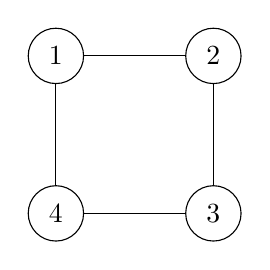
\begin{tikzpicture}
				\node[vertex] (a) at (0, 2) {$1$};
				\node[vertex] (b) at (2, 2) {$2$};
				\node[vertex] (c) at (2, 0) {$3$};
				\node[vertex] (d) at (0, 0) {$4$};
	
				\draw[edge] (a) -- (b);
				\draw[edge] (b) -- (c);
				\draw[edge] (c) -- (d);
				\draw[edge] (d) -- (a);
			\end{tikzpicture}
		\end{center}
	\end{minipage}
	\begin{minipage}{0.10\textwidth}
		\begin{center}
			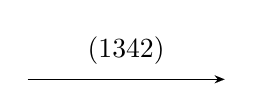
\begin{tikzpicture}
				\draw[-{Stealth[length=1.25mm, width=1mm]}, line width=0.01pt] (0,0) -- (2.5,0)
				node[midway, above=2pt] {$(1342)$};
			\end{tikzpicture}
		\end{center}
	\end{minipage}
	\begin{minipage}{0.40\textwidth}
		\begin{center}
			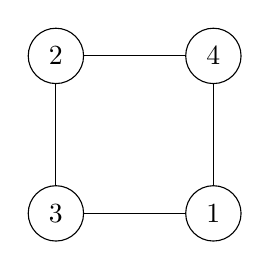
\begin{tikzpicture}
				\node[vertex] (a) at (0, 2) {$2$};
				\node[vertex] (b) at (2, 2) {$4$};
				\node[vertex] (c) at (2, 0) {$1$};
				\node[vertex] (d) at (0, 0) {$3$};
	
				\draw[edge] (a) -- (b);
				\draw[edge] (b) -- (c);
				\draw[edge] (c) -- (d);
				\draw[edge] (d) -- (a);
			\end{tikzpicture}
		\end{center}
	\end{minipage}

	\vspace{1em}

	that clearly fails to be adjacency preserving. Thus, because $(12) \in S_{4}$ and $(1234) \in D_{4}$ but $(1342) = (1234)^{(12)} \not\in D_{4}$, $D_{4} = \phi(D_{4}) = \phi(N)$ isn't closed under conjugation in $S_{4}$. Hence, $\phi(N) \not\unlhd S_{4}$ in this case.
\end{solution}

\begin{subproblem}
	Prove that if $\ker(\phi) \le N$ and $\phi(N) \unlhd H$, then $N \unlhd G$. Give an example showing that this implication is false if we drop the hypothesis that $\ker(\phi) \le N$.
\end{subproblem}

\begin{solution}
	First, we'll attempt to show that $N \unlhd G$ when $\ker(\phi) \le N$ and $\phi(N) \unlhd H$, and then reevaluate the truth of that statement when we no longer assume $\ker(\phi) \le N$. \\

	\begin{step}
		Prove the claim.
	\end{step}

	Let $n \in N$ and $g \in G$ be arbitrary elements of their respective groups. To prove the claim, we're going to want to show that everything we've assumed about $G$, $H$, $N$, and $\phi$ implies that $N \unlhd G$, or in other words, that:

	\begin{align*}
		n^{g} \in N \\
	\end{align*}

	Let's approach this by first reasoning about $\phi(n^{g})$ and then working backwards to $[n^{g}]$. By definition of conjugation, we know that:

	\begin{align*}
		\phi(n^{g}) &= \phi(g^{-1}ng) &&\text{(By definition of conjugation)} \\
	\end{align*}

	And since $\phi \colon G \rightarrow H$ is a group homomorphism, we know that $\phi(xy) = \phi(x)\phi(y)$ for all $x, y \in G$, and so:

	\begin{align*}
		\phi(n^{g}) &= \phi(g^{-1}ng) &&\text{(By definition of conjugation)} \\
		&= \phi(g^{-1})\phi(n)\phi(g) &&\text{(Since $\phi$ is a homomorphism)} \\
	\end{align*}

	To proceed, we'll take a quick detour to show that, because $\phi$ is a group homomorphism, $\phi(g^{-1}) = \phi(g)^{-1}$. Observe that, because:

	\begin{align*}
		\phi(g^{-1}) &= \phi(g^{-1})(1) &&\text{(By definition of the identity)} \\
		&= \phi(g^{-1})\phi(g)\phi(g)^{-1} &&\text{(By definition of inverses)} \\
		&= \phi(g^{-1}g)\phi(g)^{-1} &&\text{(Since $\phi$ is a homomorphism)} \\
		&= \phi(1)\phi(g)^{-1} &&\text{(By definition of inverses)} \\
	\end{align*}

	we can take advantage of the fact $\phi(1) = 1$ for all group homomorphisms to conclude that:

	\begin{align*}
		\phi(g^{-1}) &= \phi(1)\phi(g)^{-1} &&\text{(From our earlier equality)} \\
		&= (1)\phi(g)^{-1} &&\text{(Since $\phi(1) = 1$ because $\phi$ is a homomorphism)} \\
		&= \phi(g)^{-1} &&\text{(By definition of the identity)} \\
	\end{align*}

	And hence, $\phi(g^{-1}) = \phi(g)^{-1}$. So, picking up where we left off, we can now see that:

	\begin{align*}
		\phi(n^{g}) &= \phi(g^{-1})\phi(n)\phi(g) &&\text{(From our earlier equality)} \\
		&= \phi(g)^{-1}\phi(n)\phi(g) &&\text{(Since $\phi(g^{-1}) = \phi(g)^{-1}$)} \\
		&= \phi(n)^{\phi(g)} &&\text{(By definition of conjugation)} \\
	\end{align*}

	And since $\phi(N)$ was assumed to be a normal subgroup of $H$ (and clearly, $\phi(n) \in \phi(N)$ and $\phi(g) \in H$), we have that there must be some $k \in \phi(N)$ satisfying $\phi(n)^{\phi(g)} = k$ and hence:

	\begin{align*}
		\phi(n^{g}) &= k &&\text{(By our choice of $k$)} \\
	\end{align*}

	for that such $k$. By definition of membership of $\phi(N)$, we know that because $k \in \phi(N)$, there must exist some corresponding $m$ in $N$ for which $\phi(m) = k$. Thus:

	\begin{align*}
		\phi(n^{g}) = \phi(m) \\
	\end{align*}

	Following this thread, we can see that this means:

	\begin{align*}
		\phi(n^{g})\phi(m)^{-1} &= \phi(m)\phi(m)^{-1} &&\text{(Multiplying both sides by $\phi(m)^{-1}$ on the right)} \\
		\implies \phi(n^{g})\phi(m)^{-1} &= 1 &&\text{(By definition of inverses)} \\
		\implies \phi(n^{g})\phi(m^{-1}) &= 1 &&\text{(Since $\phi(m)^{-1} = \phi(m^{-1})$)} \\
		\implies \phi(n^{g}m^{-1}) &= 1 &&\text{(Since $\phi$ is a homomorphism)} \\
	\end{align*}

	Recall that the kernel of $\phi$, $\ker(\phi)$, is defined to be a subgroup of $N$. Thus, $n^{g}m^{-1}$ belonging to $\ker(\phi)$ necessitates that $n^{g}m^{-1}$ belongs to $N$ as well. Since $m$ was defined as being an element of $N$, and since $N$ must be closed under its binary operation by virtue of it being a subgroup, we can infer that:

	\begin{align*}
		(n^{g}m^{-1})(m) &\in N &&\text{(Since $N$ is a group and $n^{g}m^{-1}, m \in N$)} \\
		\implies n^{g}(m^{-1}{m}) &\in N &&\text{(By associativity)} \\
		\implies n^{g}(1) &\in N &&\text{(By definition of inverses)} \\
		\implies n^{g} &\in N &&\text{(By definition of the identity)} \\
	\end{align*}
	
	Thus, since $n \in N$ and $g \in G$ were arbitrary, $N$ is closed under conjugation! Hence, $N \unlhd G$ by definition of normality, as required.

	\begin{step}
		Show that the claim is false if we don't assume $\ker(\phi) \le N$.
	\end{step}

	We'll once again make use of a counter example to demonstrate that, in general, $N$ is not a normal subgroup of $G$ if we don't assume $\ker(\phi) \le N$. \\

	Consider letting $G$ and $H$ be the groups $S_{4}$ and $D_{4}$ respectively, $N$ be the subgroup $D_{4}$ and $\phi \colon G \rightarrow H$ be the `trivial' homomorphism defined by:

	\begin{align*}
		\phi(x) &= () \\
	\end{align*}

	It should be relatively clear that in this scenario, $\phi$ is a valid group homomorphism, $\phi(N)$ is a normal subgroup of $H$ (since the trivial subgroup is always normal), and that $\ker(\phi) = G = S_{4}$, which isn't a subgroup of $D_{4} = N$. \\

	As for $N$, we can use our trusty counter example of $(1234) \in D_{4}$ and $(12) \in S_{4}$ to conclude that because $(1234)^{(12)} = (1342)$, which isn't adjacency preserving, $N = D_{4}$ isn't closed under conjugation as a subgroup of $S_{4} = G$ and hence $N \not\unlhd G$. \\

	Thus, by counter example, the claim that $N \unlhd G$ fails to hold in general unless we additionally assume that $\ker(\phi) \le N$.
\end{solution}

%NOTE: Problem 5
\begin{problem}
	Let $G$ and $H$ be cyclic groups of order $m$, $n$ respectively. Here we will investigate the existence of injective and surjective homomorphisms from $G$ to $H$.
\end{problem}

%NOTE: Problem 5 (a)
\begin{subproblem}
	Prove that there exists a surjective homomorphism $\phi \colon G \rightarrow H$ if and only if $n | m$.
\end{subproblem}

\begin{solution}
	Let's first tackle the claim's forward direction, then try our hand at proving the reverse direction to establish the if-and-only-if relationship.

	\begin{step}
		Prove the forward direction.
	\end{step}

	The forward direction of the claim states that the existence of a surjective group homomorphism $\phi \colon G \rightarrow H$ implies that $n$ (the order of $H$) is a divisor of $m$ (the order of $G$). \\

	So, we'll naturally start by assuming such a surjective $\phi$ exists. By definition of the order of a group, we know that there must be $n$ elements in $H$. Now, let $h \in H$ be any such element. By the surjectivity of $\phi$, we know that there must exist some corresponding element, $g_{0} \in G$, for which:

	\begin{align*}
		\phi(g_{0}) &= h &&\text{(By our choice of $g_{0}$ and surjectivity of $\phi$)} \\
	\end{align*}

	Thus, we know that the fiber of $h$, $F_{h} \coloneq \set{g \in G \colon \phi(g) = h}$, is always non-empty. Drawing (heavy) inspiration from a discussion of fibers given in lecture, we'll proceed by proving that there exists some fixed integer $k \in \mathbb{Z}$ satisfying $|F_{h}| = k$ for all such $h$ in $H$. \\

	Our approach here will be to show that $F_{h}$ is equal to the right coset $\ker(\phi)g_{0}$. If we're able to do that, we'll be able to invoke Proposition 7.7 to assert that $|F_{h}| = |\ker(\phi)|$ for all $h$, and hence that the cardinality of $F_{h}$ is the same for all $h$. To that end, observe that because:

	\begin{align*}
		x \in F_{h} &\iff \phi(x) = h &&\text{(By definition of $F_{h}$)} \\
		&\iff \phi(x) = \phi(g_{0}) &&\text{(Since $\phi(g_{0}) = h$ by our choice of $g_{0}$)} \\
		&\iff \phi(x)\phi(g_{0})^{-1} = \phi(g_{0})\phi(g_{0})^{-1} &&\text{(Multiplying both sides by $\phi(g_{0})^{-1}$ on the right)} \\
		&\iff \phi(x)\phi(g_{0})^{-1} = 1 &&\text{(By definition of inverses)} \\
		&\iff \phi(x)\phi(g_{0}^{-1}) = 1 &&\text{(Since $\phi$ is a group homomorphism)} \\
		&\iff \phi(xg_{0}^{-1}) = 1 &&\text{(Since $\phi$ is a group homomorphism)} \\
	\end{align*}

	we know every element $x$ in the fiber of $h$ satisfies $\phi(xg_{0}^{-1}) = 1$. Thus, by definition of the kernel of $\phi$, we have that:

	\begin{align*}
		x \in F_{h} &\iff xg_{0}^{-1} \in \ker(\phi) &&\text{(Since $\phi(xg_{0}^{-1}) = 1$ and by definition of $\ker(\phi)$)} \\
		&\iff g_{0} \equiv x \mod{\ker(\phi)} &&\text{(By definition of congruence modulo $\ker(\phi)$)} \\
		&\iff x \in \ker(\phi)g_{0} &&\text{(By definition of $\ker(\phi)g_{0}$)} \\
	\end{align*}

	Hence, we have that for all $h \in H$, $F_{h} = \ker(\phi)g_{0}$, where $g_{0} \in G$ is a necessarily existent element in $G$ satisfying $\phi(g_{0}) = h$. And so, since we know $|F_{h}| = |\ker(\phi)g_{0}|$, and Proposition 7.7 tells us that $|\ker(\phi)g_{0}| = |\ker(\phi)|$, which is independent of $h$. Hence, letting $k = |\ker(\phi)|$ be a fixed integer, we have that $|F_{h}| = k$ for all $h$, implying that the fiber of every element in $H$ is the same size, $k$. \\

	But recall that there are $n$ elements in the codomain $H$! So, since for each of those $n$ elements, there exist exactly $k$ distinct elements $g_{1}, \ldots, g_{k} \in G$ satisfying $\phi(g_{i}) = h$ for every $1 \le i \le k$, there must be $k$ elements in $G$ for every one element in $H$. So, since $m$ was defined as the order of $G$:

	\begin{align*}
		m &= kn \\
	\end{align*}

	Hence, since $k$ is an integer, $m$ must be divisible by $n$, thus proving the claim's forward direction.

	\begin{step}
		Prove the reverse direction.
	\end{step}

	Next up, we'll need to prove the claim's reverse direction, which states that the order of $G$, $m$, being divisible by the order of $H$, $n$, implies the existence of a surjective homomorphism from $G$ to $H$. \\

	Before continuing, recall that $G$ and $H$ are cyclic groups, which by definition of cyclicity implies that there exists some $g_{0} \in G$, $h_{0} \in H$ respectively such that $\gen{g_{0}} = G$ and $\gen{h_{0}} = H$. \\

	To prove the claim, we'll take a constructivist approach by assuming $n$ divides $m$ and using that to propose a valid surjective homomorphism from $G$ to $H$. Doing just that, we'll assume that when $n$ is a divisor of $m$, the function $\phi \colon G \rightarrow H$ defined by:

	\begin{align*}
		\phi(g) &= h_{0}^{i} \text{, where } i \text{ satisfies } g_{0}^{i} = g \\
	\end{align*}

	is exactly our sought-after function. To prove this is indeed the case, we'll need to show that $\phi$ is well-defined, a group homomorphism, and surjective, each of which we'll demonstrate separately.

	\begin{step}
		$\phi$ is well-defined.
	\end{step}

	We'll begin by proving $\phi$ to be well-defined. It's not hard to see the stated domain and codomain of $\phi$ must be correct, because $\gen{g_{0}}$ equalling $G$ implies there always exists some integer $i \in \mathbb{Z}$ for which $g_{0}^{i} = g$ for any $g \in G$, and because $h_{0}^{i} \in H$. \\

	However, to fully conclude the well-definedness of $\phi$, we'll need to show that our choice of $i$ doesn't affect what $\phi(g)$ equals. To that end, let $g \in G$ be arbitrary, and let $i, j \in \mathbb{Z}$ be two integers satisfying $g_{0}^{i} = g$ and $g_{0}^{j} = g$. We'll want to show that this therefore implies $h_{0}^{i} = h_{0}^{j}$. \\

	Recall from earlier that $n$ is assumed to be a divisor of $m$. Hence there exists some $k \in \mathbb{Z}$ such that $m = kn$. By doing some slight massaging, we can see that:

	\begin{align*}
		g_{0}^{i} &= g_{0}^{j} &&\text{(By our choice of $i$ and $j$)} \\
		\implies g_{0}^{i}(g_{0}^{j})^{-1} &= g_{0}^{j}(g_{0}^{j})^{-1} &&\text{(Multiplying both sides by $(g_{0}^{j})^{-1}$ on the right)} \\
		\implies g_{0}^{i}(g_{0}^{j})^{-1} &= 1 &&\text{(By definition of inverses)} \\
		\implies g_{0}^{i}g_{0}^{-j} &= 1 &&\text{(By exponent laws)} \\
		\implies g_{0}^{i-j} &= 1 &&\text{(By exponent laws)} \\
	\end{align*}

	Because $g_{0}$ is the generator of $G$, a group of order $m$, we know it too must have an order of $m$. Hence, by Theorem 4.3, we know that $g_{0}^{i-j}$ equalling 1 implies $m$ divides $i - j$. Thus, there exists some integer $\ell \in \mathbb{Z}$ such that:

	\begin{align*}
		\ell m &= i - j &&\text{(By our choice of $\ell$)} \\
		\implies i &= \ell m + j &&\text{(Rearranging)} \\
	\end{align*}

	And so since $kn = m$:

	\begin{align*}
		i &= \ell m + j &&\text{(From our earlier equality)} \\
		\implies i &= \ell kn + j &&\text{(Since $m = kn$)} \\
	\end{align*}

	So:

	\begin{align*}
		h_{0}^{i} &= h_{0}^{\ell kn + j} &&\text{(By our characterization of $i$)} \\
		&= h_{0}^{\ell kn}h_{0}^{j} &&\text{(By exponent laws)} \\
		&= (h_{0}^{n})^{\ell k}h_{0}^{j} &&\text{(By exponent laws)} \\
	\end{align*}

	And because $\ord{h_{0}} = n$ for the same reason $\ord{g_{0}} = m$, we can finally conclude that:

	\begin{align*}
		h_{0}^{i} &= (h_{0}^{n})^{\ell k}h_{0}^{j} &&\text{(From our earlier equality)} \\
		&= (1)^{\ell k}h_{0}^{j} &&\text{(By definition of order and since $\ord{h_{0}} = n$)} \\
		&= (1)h_{0}^{j} &&\text{(Inductively by definition of the identity)} \\
		&= h_{0}^{j} &&\text{(By definition of the identity)} \\
	\end{align*}

	Cementing that $\phi$ is indeed a well-defined function from $G$ to $H$.

	\begin{step}
		$\phi$ is homomorphic.
	\end{step}

	To show that $\phi$ is a homomorphism, we'll need to prove that $\phi(xy) = \phi(x)\phi(y)$ for all $x$ and $y$ in $\phi$'s domain. So, let $g_{1}, g_{2} \in G$ such that $g_{1} = g_{0}^{i}$ and $g_{2} = g_{0}^{j}$ for two necessarily existent integers $i$ and $j$ in $\mathbb{Z}$. \\

	Because:

	\begin{align*}
		\phi(g_{1}g_{2}) &= \phi(g_{0}^{i}g_{0}^{j}) &&\text{(By our characterization of $g_{1}$ and $g_{2}$)} \\
		&= \phi(g_{0}^{i+j}) &&\text{(By exponent laws)} \\
		&= h_{0}^{i+j} &&\text{(By definition of $\phi$)} \\
		&= h_{0}^{i}h_{0}^{j} &&\text{(By exponent laws)} \\
		&= \phi(g_{0}^{i})\phi(g_{0}^{j}) &&\text{(By definition of $\phi$)} \\
		&= \phi(g_{1})\phi(g_{2}) &&\text{(By our characterization of $g_{1}, g_{2}$)} \\
	\end{align*}

	we have that $\phi(g_{1}g_{2}) = \phi(g_{1})\phi(g_{2})$ for arbitrary $g_{1}, g_{2} \in G$, making $\phi$ a homomorphism.

	\begin{step}
		Prove that $\phi$ is surjective.
	\end{step}

	Last but not least, we'll need to show that $\phi$ is surjective. So let $h \in H$ be arbitrary. Because of $h_{0}$'s status as a generator for $H$, we know that there exists some $i \in \mathbb{Z}$ for which $h_{0}^{i} = h$. Clearly, since $G$ is a group and $g_{0} \in G$, we know that there must exist some $g \in G$ such that $g = g_{0}^{i}$. But because this means:

	\begin{align*}
		\phi(g) &= \phi(g_{0}^{i}) &&\text{(By definition of $g$)} \\
		&= h_{0}^{i} &&\text{(By definition of $\phi$)} \\
		&= h &&\text{(By our characterization of $h$)} \\
	\end{align*}

	we have that every element $h$ in $H$ has some corresponding element $g \in G$ such that $\phi(g) = h$. Thus, $\phi$ is surjective. \\

	Therefore, by the results of \textbf{(III)}, \textbf{(IV)}, and \textbf{(V)}, $\phi$ is a well-defined homomorphic surjection from $G$ to $H$, and because its existence is implied by the assumptions made by the claim's reverse direction, this direction is necessarily proven. \\

	Thus, since the claim's forward and reverse directions have been independently proven by \textbf{(I)} and \textbf{(II)}, the claim's if-and-only-if relationship has been rigorously established.
\end{solution}

%NOTE: Problem 5 (b)
\begin{subproblem}
	Suppose that there exists an injective homomorphism $\psi \colon G \rightarrow H$. What can be said about the relationship between $m$ and $n$? Formulate and prove a proposition similar to the result of part \textbf{(a)}. Make sure your proposition is an ``if and only if'', and prove both directions.
\end{subproblem}

\begin{solution}
	We'll propose that for cyclic groups $G$ and $H$ of orders $m$ and $n$ respectively, that the statement: \\

	``There exists an injective homomorphism $\psi \colon G \rightarrow H$ if and only if $m$ divides $n$.'' \\

	holds. To prove that this statement is actually true, we'll prove both the forward and reverse directions of the above claim independently.

	\begin{step}
		Prove the forward direction.
	\end{step}

	The forward direction of the claim amounts to the assertion that, should an injective homomorphism $\psi$ exist from $G$ to $H$, then $m$ must divide $n$. To prove this is the case, we'll need to show there exists some integer $k \in \mathbb{Z}$ such that $km = n$. Thankfully, as we'll soon see, this isn't very hard to do. \\

	Consider the image of $\psi$, $\text{im}(\psi)$. By Proposition 8.6, we know that $\text{im}(\psi)$ is a subgroup of $H$, which means by Lagrange's theorem that $|\text{im}(\psi)|$ must be a divisor of $|H|$, which we defined to be $n$. Hence, there exists some integer $k \in \mathbb{Z}$ such that $k|\text{im}(\psi)| = n$. \\

	By the injectivity of $\psi$, we know that for any two distinct $g_{1}$ and $g_{2}$ belonging to $G$, $\psi(g_{1}) \neq \psi(g_{2})$. Recall however that the definition of the image of $\psi$ is really just the image of $G$ under $\psi$, or in other words:

	\begin{align*}
		\text{im}(\psi) &= \set{h \in H \colon \text{there exists some} \; g \in G \; \text{such that} \; \psi(g) = h} &&\text{(By definition of $\psi$)} \\
	\end{align*}

	And since there is exactly one such $h$ in $H$ for every $g$ in $G$ by the injectivity of $\psi$, and because there are $|G| = m$ elements in $G$, we have that $|\text{im}(\psi)| = |G| = m$. Hence, since we determined that $k|\text{im}(\psi)| = n$ earlier, we have that:

	\begin{align*}
		k|\text{im}(\psi)| &= n &&\text{(From our earlier equality)} \\
		\implies km &= n &&\text{(Since $|\text{im}(\psi)| = |G| = m$)} \\
	\end{align*}

	Thus proving that $m$ is a divisor of $n$ and thereby the forward direction of the claim.

	\begin{step}
		Prove the reverse direction.
	\end{step}

	To prove the claim's reverse direction, which states that $m$ being a divisor of $n$ implies the existence of an injective homomorphism from $G$ to $H$, we'll once again take the `constructivist' approach. \\

	So, let's now assume that $m$ divides $n$ and hence that there exists some integer $k \in \mathbb{Z}$ such that $n = mk$. Recalling that $G$ and $H$ were both given to be cyclic groups, we'll also use the implied existence of generators $g_{0} \in G$ and $h_{0} \in H$ satisfying $\gen{g_{0}} = G$ and $\gen{h_{0}} = H$ for the remainder of our proof. \\

	To complete the proof, we'll show that the function $\psi \colon G \rightarrow H$ defined by:

	\begin{align*}
		\psi(g) &= h_{0}^{ki} \text{, where } i \text{ is an integer satisfying } g_{0}^{i} = g \\
	\end{align*}

	is a well-defined, homomorphic injection from $G$ to $H$. We devote some time to showing the validity of each of those statements regarding $\psi$ below:

	\begin{step}
		Prove $\psi$ is well-defined.
	\end{step}

	Immediately, it should not be hard to see that the stated domain and co-domain of $\psi$ is correct, since $g_{0}$ being defined as a generator of $G$ necessitates the existence of an integer $i$ such that $g_{0}^{i} = g$ for all $g$ in $G$, and because $h_{0}$ being an element of the group $H$ requires that $h_{0}^{ik} \in H$ for all $k$ and $i$ as well. \\

	To solidify that $\psi$ is indeed well-defined, we'll also show that the specific choice of $i$ made, so long as it satisfies $g_{0}^{i} = g$, won't affect the value of $\psi(g)$. \\

	To that end, let $g \in G$ be arbitrary, and let $i$ and $j$ be any two integers satisfying $g_{0}^{i} = g$ and $g_{0}^{j} = g$. We'll now need to show that $h_{0}^{ik} = h_{0}^{jk}$. Thankfully this isn't too hard to see. Echoing our findings in attempting to prove the reverse direction in part \textbf{(a)} of this problem, we know that $g_{0}^{i}$ and $g_{0}^{j}$ both equalling $g$ implies that $i = \ell m + j$ for some integer $\ell \in \mathbb{Z}$. And so, since:

	\begin{align*}
		h_{0}^{ik} &= h_{0}^{(\ell m + j)k} &&\text{(By our characterization of $i$)} \\
		&= h_{0}^{\ell mk + jk} &&\text{(By distributivity of multiplication over addition)} \\
		&= h_{0}^{\ell mk}h_{0}^{jk} &&\text{(By exponent laws)} \\
		&= (h_{0}^{mk})^{\ell}h_{0}^{jk} &&\text{(By exponent laws)} \\
		&= (h_{0}^{n})^{\ell}h_{0}^{jk} &&\text{(Since $mk = n$ by our choice of $k$)} \\
		&= (1)^{\ell}h_{0}^{jk} &&\text{(Since $\ord{h_{0}} = n$ because $|H| = n$ and $\gen{h_{0}} = H$)} \\
		&= (1)h_{0}^{jk} &&\text{(Inductively by definition of the identity)} \\
		&= h_{0}^{jk} &&\text{(By definition of the identity)} \\
	\end{align*}

	we have that $h_{0}^{ik} = h_{0}^{jk}$ and hence $\psi$ is a well-defined function.

	\begin{step}
		Prove $\psi$ is homomorphic.
	\end{step}

	To show that $\psi$ is a homomorphism, we need to show that for all $x, y \in G$, $\psi(xy) = \psi(x)\psi(y)$. \\

	So, let's let $g_{1}, g_{2} \in G$ be arbitrary elements and let $i$ and $j$ be two (necessarily existent integers) satisfying $g_{1} = g_{0}^{i}$ and $g_{2} = g_{0}^{j}$. Carrying out the necessary computations, we have that:

	\begin{align*}
		\psi(g_{1}g_{2}) &= \psi(g_{0}^{i}g_{0}^{j}) &&\text{(By our characterization of $g_{1}, g_{2}$)} \\
		&= \psi(g_{0}^{i+j}) &&\text{(By exponent laws)} \\
		&= h_{0}^{(i+j)k} &&\text{(By definition of $\psi$)} \\
		&= h_{0}^{ik + jk} &&\text{(By distributivity of multiplication over addition)} \\
		&= h_{0}^{ik}h_{0}^{jk} &&\text{(By exponent laws)} \\
		&= \psi(g_{0}^{i})\psi(g_{0}^{j}) &&\text{(By definition of $\psi$)} \\
		&= \psi(g_{1})\psi(g_{2}) &&\text{(By our characterization of $g_{1}, g_{2}$)} \\
	\end{align*}

	And hence $\psi(g_{1}g_{2}) = \psi(g_{1})\psi(g_{2})$, proving that $\psi$ is a homomorphism.

	\begin{step}
		Prove that $\psi$ is injective.
	\end{step}

	Finally, we arrive at the last claim made about $\psi$, that being that it constitutes an injection from $G$ to $H$. \\

	To see why this is the case, we'll let $g_{1}, g_{2} \in G$ be arbitrary elements of $G$ and $i$ and $j \in \mathbb{Z}$ be integers such that $g_{1} = g_{0}^{i}$ and $g_{2} = g_{0}^{j}$ once again. What we want to do is show that if $\psi(g_{1}) = \psi(g_{2})$, then that must mean $g_{1} = g_{2}$ as well. So, assuming it is indeed the case that $\psi(g_{1}) = \psi(g_{2})$, we can see by the following logic:

	\begin{align*}
		\psi(g_{1}) &= \psi(g_{2}) &&\text{(By assumption)} \\
		\implies \psi(g_{0}^{i}) &= \psi(g_{0}^{j}) &&\text{(By our characterization of $g_{1}$ and $g_{2}$)} \\
		\implies h_{0}^{ik} &= h_{0}^{jk} \\
	\end{align*}

	Which, drawing on a similar observation made earlier about what happens when $g_{0}^{i} = g_{0}^{j}$, implies that there must exist some integer $\ell$ such that $ik = \ell n + jk$. Hence, we have that $\ell n = ik - jk$. But remember! $m$ is assumed to be a divisor of $n$ satisfying $n = mk$. So, we know:

	\begin{align*}
		\ell n &= ik - jk &&\text{(From our earlier equality)} \\
		\implies \ell km &= ik - jk &&\text{(Since $n = mk$)} \\
		\implies \ell m &= i - j &&\text{(Dividing both sides by $k$)} \\
		\implies i &= \ell m + j &&\text{(Rearranging)} \\
	\end{align*}

	And thus, we may conclude:

	\begin{align*}
		g_{1} &= g_{0}^{i} &&\text{(By our characterization of $g_{1}$)} \\
		&= g_{0}^{\ell m + j} &&\text{(By our characterization of $i$)} \\
		&= g_{0}^{\ell m}g_{0}^{j} &&\text{(By exponent laws)} \\
		&= (g_{0}^{m})^{\ell}g_{0}^{j} &&\text{(By exponent laws)} \\
		&= (1)^{\ell}g_{0}^{j} &&\text{(By definition of order and since $\ord{g_{0}} = m$ because $\gen{g_{0}} = G$)} \\
		&= (1)g_{0}^{j} &&\text{(Inductively by definition of the identity)} \\
		&= g_{0}^{j} &&\text{(By definition of the identity)} \\
		&= g_{2} &&\text{(By our characterization of $g_{2}$)} \\
	\end{align*}

	Hence, because $\psi(g_{1}) = \psi(g_{2})$ implies that $g_{1} = g_{2}$, $\psi$ is an injective function. \\

	Thus, by \textbf{(III)}, \textbf{(IV)}, and \textbf{(V)}, we have that our proposed $\psi$ is a well-defined, homomorphic injection from $G$ to $H$. Hence, the reverse direction is proven. \\

	And so, since \textbf{(I)} and \textbf{(II)} both show the claim's forward and reverse directions hold, we've successfully proven the proposition we came up with!
\end{solution}

%FIX: Problem 6
\begin{problem}
	Determine whether each of the following isomorphisms are correct. If correct, prove it by either explicitly constructing an isomorphism or using results from the lecture notes. If incorrect, prove an isomorphic invariant that distinguishes the two groups, or directly proving that no isomorphism can exist.
\end{problem}

%NOTE: Problem 6 (a)
\begin{subproblem}
	$\mathbb{Z}_{18} \simeq \mathbb{Z}^{\times}_{27}$.
\end{subproblem}

\begin{solution}
	This isomorphism is correct. \\

	Since:

	\vspace{1em}

	\begin{tabularx}{\linewidth}{Y Y Y}
		$\gcd(0, 27) = 27$ & $\gcd(9, 27) = 3$ & $\gcd(18, 27) = 3$ \\[8pt]
		$\boxed{\gcd(1, 27) = 1}$ & $\boxed{\gcd(10, 27) = 1}$ & $\boxed{\gcd(19, 27) = 1}$ \\[8pt]
		$\boxed{\gcd(2, 27) = 1}$ & $\boxed{\gcd(11, 27) = 1}$ & $\boxed{\gcd(20, 27) = 1}$ \\[8pt]
		$\gcd(3, 27) = 3$ & $\gcd(12, 27) = 3$ & $\gcd(21, 27) = 3$ \\[8pt]
		$\boxed{\gcd(4, 27) = 1}$ & $\boxed{\gcd(13, 27) = 1}$ & $\boxed{\gcd(22, 27) = 1}$ \\[8pt]
		$\boxed{\gcd(5, 27) = 1}$ & $\boxed{\gcd(14, 27) = 1}$ & $\boxed{\gcd(23, 27) = 1}$ \\[8pt]
		$\gcd(6, 27) = 3$ & $\gcd(15, 27) = 3$ & $\gcd(24, 27) = 3$ \\[8pt]
		$\boxed{\gcd(7, 27) = 1}$ & $\boxed{\gcd(16, 27) = 1}$ & $\boxed{\gcd(25, 27) = 1}$ \\[8pt]
		$\boxed{\gcd(8, 27) = 1}$ & $\boxed{\gcd(17, 27) = 1}$ & $\boxed{\gcd(26, 27) = 1}$ \\[8pt]
	\end{tabularx}

	\vspace{1em}

	We have by Proposition 1.7 that $\mathbb{Z}^{\times}_{27} = \set{1, 2, 4, 5, 7, 8, 10, 11, 13, 14, 16, 17, 19, 20, 22, 23, 25, 26}$. Thus, $\mathbb{Z}^{\times}_{27}$ is clearly a finite group of order 18. Thanks to Proposition 9.4, one way for us to show that $\mathbb{Z}^{\times}_{27}$ is isomorphic to $\mathbb{Z}_{18}$ would be for us to show that $\mathbb{Z}^{\times}_{27}$ is cyclic, which we can do by finding a generator for $\mathbb{Z}^{\times}_{27}$. \\

	With that in mind, we'll propose that $2$ is a valid generator for $\mathbb{Z}^{\times}_{27}$. To prove this is indeed the case, we'll present both a clever and brute force approach. \\

	The cleverer method is to make use of Corollary 7.9, which tells us that the order of $2$ in $\mathbb{Z}^{\times}_{27}$ must be a divisor of $|\mathbb{Z}^{\times}_{27}| = 18$. Thus, we know $\ord{2} = 1, 2, 3, 6, 9$, or $18$. Clearly $2 \neq 1 $, so $\ord{2}$ cannot be 1, and since:
	\vspace{1em}

	\begin{tabularx}{\linewidth}{Y Y}
		$(2)^{2} \equiv 4 \mod{27}$ & $2^{6} \equiv 10 \mod{27}$ \\
		$(2)^{3} \equiv 8 \mod{27}$ & $2^{9} \equiv 26 \mod{27}$ \\
	\end{tabularx}

	\vspace{1em}

	$\ord{2}$ cannot be 2, 3, 6, or 9 either, since $2$ raised to the power of any of those numbers doesn't equal one, which is a prerequisite for that integer to be the order of 2. Thus, that simply leaves us with 18 as the only possibility for the order of $2$. Thus, we know that the order of the subgroup generated by 2, $\gen{2}$, must be 18 as well by Corollary 4.4, and hence $\gen{2} = \mathbb{Z}^{\times}_{27}$. \\

	Thus, since $\mathbb{Z}^{\times}_{27}$ contains a generator of itself, it is indeed cyclic. \\

	Using the brute force approach for further confirmation, we can see that because:

	\vspace{1em}

	\begin{tabularx}{\linewidth}{Y Y}
		$2^{1} \equiv 2 \mod{27}$ & $2^{10} \equiv 25 \mod{27}$ \\
		$2^{2} \equiv 4 \mod{27}$ & $2^{11} \equiv 23 \mod{27}$ \\
		$2^{3} \equiv 8 \mod{27}$ & $2^{12} \equiv 19 \mod{27}$ \\
		$2^{4} \equiv 16 \mod{27}$ & $2^{13} \equiv 11 \mod{27}$ \\
		$2^{5} \equiv 5 \mod{27}$ & $2^{14} \equiv 22 \mod{27}$ \\
		$2^{6} \equiv 10 \mod{27}$ & $2^{15} \equiv 17 \mod{27}$ \\
		$2^{7} \equiv 20 \mod{27}$ & $2^{16} \equiv 7 \mod{27}$ \\
		$2^{8} \equiv 13 \mod{27}$ & $2^{17} \equiv 14 \mod{27}$ \\
		$2^{9} \equiv 26 \mod{27}$ & $2^{18} \equiv 1 \mod{27}$ \\
	\end{tabularx}

	\vspace{1em}

	we have both that $\ord{2} = 18$ and $\gen{2} = \mathbb{Z}^{\times}_{27}$. \\

	Therefore, $\mathbb{Z}^{\times}_{27}$ is indeed a cyclic group of order 18 and is thus isomorphic to $\mathbb{Z}_{18}$ by Proposition 9.4. But wait! The problem asks us if $\mathbb{Z}_{18}$ is isomorphic to $\mathbb{Z}^{\times}_{27}$, not if $\mathbb{Z}^{\times}_{27}$ is isomorphic to $\mathbb{Z}_{18}$, shouldn't that be a problem? No little one. Proposition 9.1 (b) has us covered. Since we've managed to conclude $\mathbb{Z}^{\times}_{27} \simeq \mathbb{Z}_{18}$, we automatically have that $\mathbb{Z}_{18} \simeq \mathbb{Z}^{\times}_{27}$ by symmetry of $\simeq$. \\

	Thus, the isomorphism holds.
\end{solution}

%FIX: Problem 6 (b)
\begin{subproblem}
	$A_{4} \simeq S_{3} \times \mathbb{Z}_{2}$.
\end{subproblem}

\begin{solution}
	This isomorphism is \underline{not} correct. \\

	To prove this, we'll show that the existence of an order 6 element in $S_{3} \times \mathbb{Z}_{2}$, and the absence of one in $A_{4}$, precludes the two groups from being isomorphic to one another. We'll demonstrate each of these claims separately.

	\begin{step}
		Prove $S_{3} \times \mathbb{Z}_{2}$ has an element of order 6.
	\end{step}

	Here, we can rely on the fact that, since $\ord{(123)} = 3$ in $S_{3}$, and $\ord{1} = 2$ in $\mathbb{Z}_{2}$, we can deduce that $\ord{((123), 1)} = \lcm{3}{2} = 6$. Once again using brute force:

	\vspace{1em}

	\begin{tabularx}{\linewidth}{Y Y}
		$((123), 1)^{1} = ((123), 1)$ & $((123), 1)^{4} = ((123), 0)$ \\
		$((123), 1)^{2} = ((132), 0)$ & $((123), 1)^{5} = ((132), 1)$ \\
		$((123), 1)^{3} = ((), 1)$ & $((123), 1)^{6} = ((), 0)$ \\
	\end{tabularx}

	\vspace{1em}

	we can see that $((123), 1)$ is indeed an order 6 element of $S_{3} \times \mathbb{Z}_{2}$.

	\begin{step}
		Prove $A_{4}$ doesn't have any elements of order 6.
	\end{step}

	To show $A_{4}$ doesn't have any element of order 6, we'll try and reason about the notion directly as opposed to brute-forcing every one of its 12 elements.

	\begin{itemize}
		\item $A_{4}$ isn't isomorphic to $S_{3} \times \mathbb{Z}_{2}$ since $S_{3} \times \mathbb{Z}_{2}$ contains an element of order 6, but $A_{4}$ doesn't
	\end{itemize}
\end{solution}

%FIX: Problem 6 (c)
\begin{subproblem}
	$\dprod{6}{15} \simeq \dprod{3}{30}$.
\end{subproblem}

\begin{solution}
	\begin{itemize}
		\item Pretty sure false. B/c $\dprod{3}{30}$ isn't cyclic whereas $\dprod{6}{15}$ is, but IDK
		\begin{itemize}
			\item Maybe has to do with gcd, may have been proven in tut
		\end{itemize}
	\end{itemize}
\end{solution}

%FIX: Problem 6 (d)
\begin{subproblem}
	$\mathbb{Q} \times \mathbb{Q} \simeq \mathbb{Q}$.
\end{subproblem}

\begin{solution}
	\begin{itemize}
		\item Highkey true heuristically
	\end{itemize}
\end{solution}

\ifdefined\iscombined
	\newpage
\else
	\end{document}
\fi
